\documentclass[a4paper,11pt]{article}
\usepackage[french]{babel}
\usepackage[T1]{fontenc}
\usepackage[utf8]{inputenc}
\usepackage{lmodern}
\usepackage{microtype}
\usepackage{hyperref}
\usepackage{graphicx}
\usepackage{booktabs}
\usepackage{standalone}
\usepackage{enumitem}
\usepackage{wrapfig}


\begin{document}

\begin{titlepage}

  \begin{center}

    \begin{figure}[!htbp]
    \centering
    
\includegraphics[width=10cm]{Img/image1.png}
    \end{figure}

    \Large{\textbf{Rapport du projet intégrateur}} \\
    \Large{\textbf{BANG "le jeu de dés"}} \\

    \begin{figure}[!htbp]
    \centering
    
\includegraphics[width=8cm]{Img/image3.jpg}
    \end{figure}

  \end{center}

  \newpage

\end{titlepage}

\tableofcontents
\newpage


\section{Introduction}

Dans le cadre de l’enseignement “Projet intégrateur”, il nous a été demandé de mener à bien une adaptation numérique d’un jeu de société. Nous avons donc commencé par la recherche de jeux potentiels à développer. \\

Il nous fallait faire un choix stratégique. En effet, celui-ci devait nous donner la possibilité de mettre en pratique nos connaissances de façon stimulante et devait être réaliste, respectant ainsi les contraintes de temps imposées. Celui-ci s’est finalement arrêté sur “Bang! Le jeu de dés”. \\

Nous avons donc planifié l’organisation afin d’estimer le temps nécessaire à la programmation de chaque fonctionnalité du projet. Chacun s’est vu attribuer des fonctions dans le but de franchir toutes les étapes de conception d’un projet informatique et d’aboutir sur un produit fini et commercialisable. \\

 Tout d’abord, nous expliquerons la structure organisationnelle que nous avons mis en place afin de mener à bien ce projet. Nous aborderons ensuite le détail de l’implémentation des différents modules du jeu (noyau, interface homme-machine, réseau, base de données) et la manière dont ils interagissent entre eux. Enfin, nous conclurons ce rapport en évoquant les améliorations possibles et les éventuelles fonctionnalités futures. \\

\newpage

\section{L'organisation}

\subsection{La technologie choisie}

Le choix de la technologie fut une décision majeure dans la réalisation du projet. Il nous fallait choisir un moyen de minimiser les conflits entre les différentes parties. En effet, ce projet regroupe plusieurs modules très différents qu’il nous a fallu unifier. \\

Nous avons choisi d’utiliser Godot Engine. L’utilisation de ce dernier peut être justifié par sa liberté de droit et sa compatibilité avec les trois systèmes d’exploitations majeurs: Linux, Windows et mac OS X. Nous avons également apprécié son environnement de développement, particulièrement efficace, notamment sur les rendus visuels et les fonctionnalités d’exportation vers un autre environnement. \\

Ce moteur de jeu permet de mettre en place différentes scènes, celles-ci étant un ensemble de nœuds organisés en arbre. Ces nœuds peuvent représenter de multiples objets qui, dans notre cas, se matérialisent en cartes, en dés, en boutons, etc… \\

Afin de programmer le comportement de ces nœuds, il est également possible de leur attacher un script ou de réutiliser une scène créée au préalable, en tant que nœud d’une autre scène. Ce système permet alors d’imbriquer des scènes les unes dans les autres, et donc de pouvoir répartir le travail. \\

Le langage principalement utilisé dans Godot Engine est le GDScript qui est un langage spécifiquement conçu pour l’environnement de Godot. Il est possible d’utiliser d’autres langages comme le C++, C\#, Python, Nim ou D. \\
 
La syntaxe de GDScript est proche de celle de Python et est relativement facile à comprendre et apprendre. Nous avons choisi d’écrire nos scripts dans ce langage conçu pour faire fonctionner l’intégralité des bibliothèques godot, nous donnant ainsi l’assurance d’une compatibilité entre nos différentes parties. 


\subsection{Le planning}
\subsubsection{L'ordre logique du code}

Nous nous sommes orientés vers la réalisation d’un jeu en ligne exclusivement multijoueur. Notre jeu est donc découpé en deux exécutables, l’un faisant office de serveur, et l’autre d’interface-utilisateur. Cela permet d’assurer la viabilité des échanges entre un joueur et le noyau. 

\newpage

Le réseau étant le seul à communiquer avec le noyau, il assure donc la sécurité du jeu, et permet la mise en place d’une structure plus résistante aux attaques. \\

Ce choix comporte des contraintes. Chaque utilisateur devra se munir d’un appareil et d’une connectique suffisamment puissante afin d’éviter les latences. Le serveur, lui aussi, demande une attention particulière et quotidienne pour son bon fonctionnement. Dans le cas d’une application réelle du jeu, il faudrait recruter une équipe réseau assurant la bonne fonctionnalité du serveur. Mais dans notre cadre scolaire, ceci ne sera pas nécessaire.  \\

Dans les premières semaines nous avons commencé à coder les fonctionnalités du jeu (le noyau, en parallèle de coder l’affichage du jeu, l’IHM). Notre but était d’avoir un noyau stable et fonctionnel avant tout. Quant à l’IHM, nous avons commencé par implémenter les dés au milieu du plateau, ainsi que les joueurs autour de la table. \\

	Une fois le noyau fonctionnel (hormis les personnages à capacité spéciale), nous avons commencé à travailler sur le réseau. Après plusieurs recherches, nous avons compris que le réseau se servait des arbres dans l’IHM et qu’il nous en fallait donc une plus aboutie que celle que nous avions à ce moment-là. \\

Nous avons donc mis plus de moyens afin d’accélérer sa programmation. Une fois que nous avions une IHM suffisamment construite, nous avons pu commencer le réseau. La mise en place du réseau fut assez longue. En effet l’IHM et l’équipe réseau devaient se synchroniser afin de mettre en place les modifications nécessaires au réseau en limitant l’attente. \\

Pendant la programmation du réseau, nous avons consacré quelques semaines à la création de la base de données liée au jeu. Celle-ci nous permet la création de comptes utilisateurs et les statistiques qui leurs sont liées, telles que le nombre de victoires ou de défaites. \\

	Une fois le réseau terminé, nous nous sommes concentrés sur les corrections de bugs. Nous avons également testé l’exportation, et apporté de nouvelles améliorations  à l’interface afin de la rendre plus agréable et compréhensible. Nous avons fini par intégrer la BDD lorsque l’aspect technique du jeu fut finalisé et présentable. \\ 

En dernier, nous avons procédé à l’exportation du projet avec de légères adaptations grâce à l’outil d'exportation intégré à Godot Engine.


\subsubsection{Le Gantt}
Voici la première version de notre Gantt, faite aux prémices du projet :\\\\
\begin{center}
	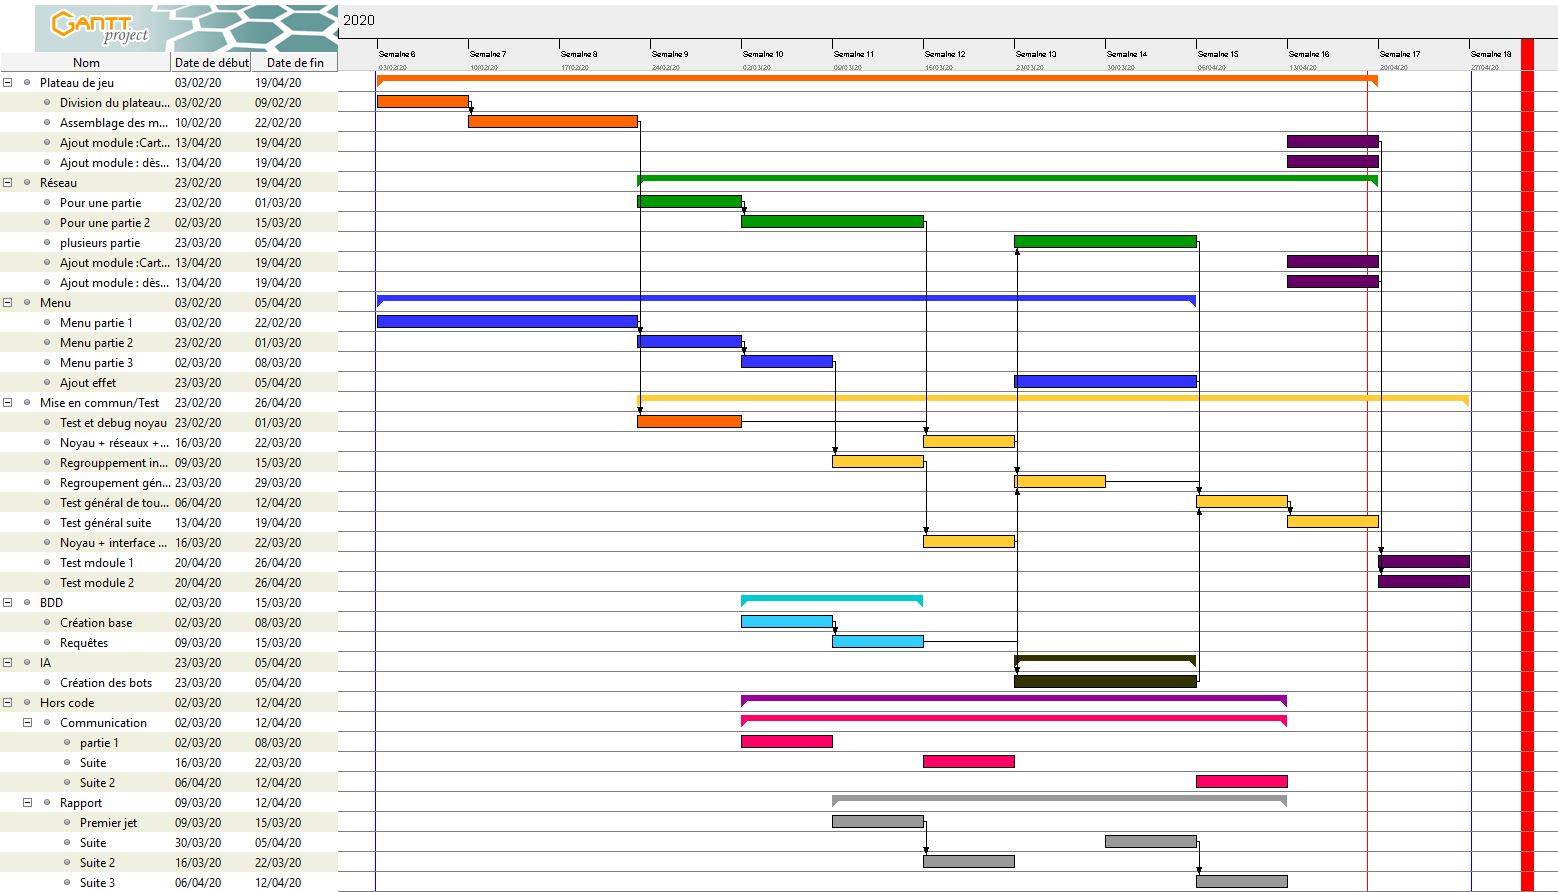
\includegraphics[width=14cm]{Img/image6.png} \\
\end{center}


Et voici la dernière version qui fut appliquée le long du projet : \\\\\\
\begin{center}
	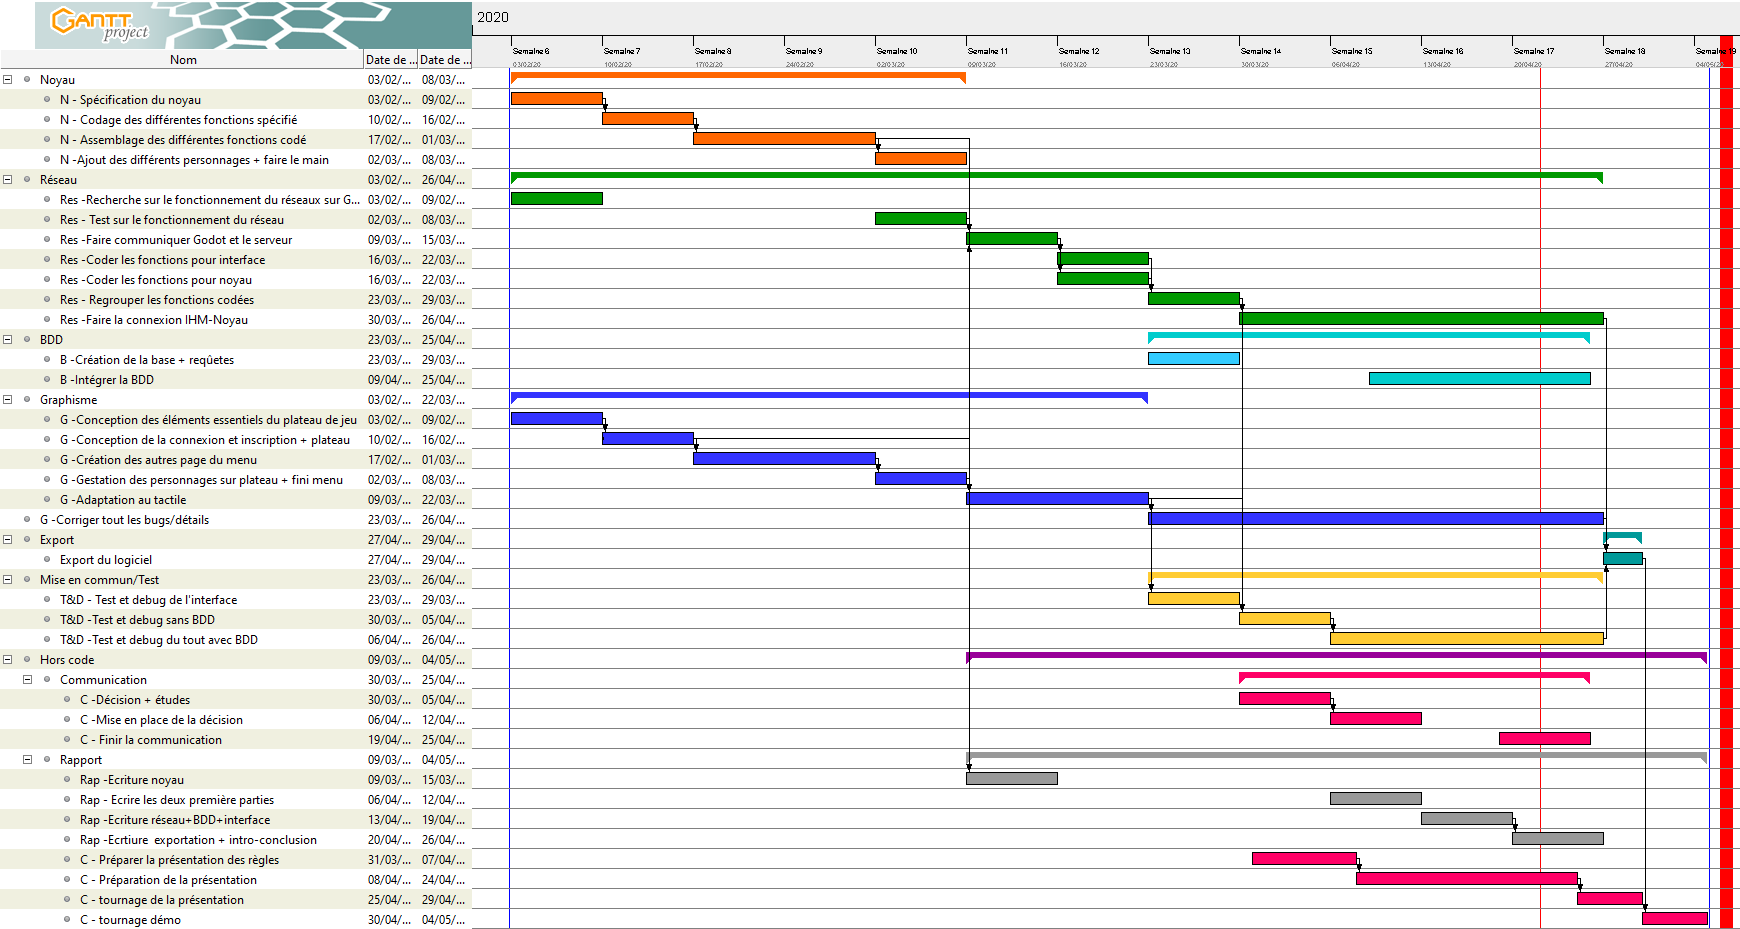
\includegraphics[width=14cm]{Img/image2.png}
\end{center}


Nous pouvons constater beaucoup de changements entre ces deux Gantt. En premier temps, certains modules, tels que ceux du noyau ou du réseau, ont prit plus de temps que prévu. En conséquence, nous avons dû raccourcir ou supprimer d’autres modules. \\

Les extensions du jeu (qui étaient optionnelles) et l'intelligence artificielle furent donc supprimées. En constatant le retard accumulé, nous avons enlevé l’implémentation d’un lobby et la gestion de plusieurs parties simultanées.  \\

Néanmoins, après avoir estimé que cet ajout ne serait pas d’une grande complexité, cette dernière fonctionnalité a pu être réalisée par l’équipe réseau en moins de temps qu’escompté. \\

Enfin, suite à la crise sanitaire du coronavirus et le changement des modalités d’évaluation, causant l’impossibilité de faire une démonstration en présentiel, nous avons dû intégrer, dans l’organisation, le tournage des différentes vidéos qui serviront à présenter notre projet. 

\subsection{Difficultés et solutions}

Nous avons rencontré plusieurs difficultés pendant ce projet. Premièrement, le choix d’utiliser une technologie que nous ne maîtrisons pas nous a contraints à l’étudier. Nous avons pu ainsi découvrir des pratiques de programmation différentes et enrichissantes d’un point de vue académique. La multitude de documentation fournie par l’entreprise de ce moteur de jeu nous a permis d’en appréhender les concepts. \\

Cependant, ce projet comportant des modules réseau et de base de données, nous devons approfondir nos connaissances sur les fonctionnalités de Godot dans ces domaines là. Les informations que nous recherchons étant moins nombreuses sur internet nous avons pris plus de temps afin de comprendre leur fonctionnement. Par exemple, l’implémentation d’un serveur centralisé ne comportait que très peu de documentation, qui était plutôt axée sur le schéma “peer-to-peer”. \\

À l’aide de dépots Git et de quelques tutoriels traitant de la question, nous avons finalement pu rassembler assez d’expérience, nous permettant ainsi de procéder à l’élaboration de ce serveur. \\

	Cette contrainte nous a malheureusement retardés dans nos différentes tâches, allongeant de ce fait le planning initial. Comme exprimé plus haut, nous avons dû pallier ce retard par une suppression de fonctionnalités moins pertinentes. \\

Le confinement nous a perturbé au début étant donné les nombreuses questions que nous nous sommes posées, une fois que tout fut clair les activités ont pu reprendre. Cependant, certains étudiants ayant une connexion instable à leur domicile, n’ont pas pu fournir un travail continu. Cette condition entraîne également une perte de concentration, notamment pour ceux possédant une famille nombreuse et/ou la garde d’enfants en bas-âge.


\subsection{Le groupe}

\subsubsection{Le rôle de la cheffe de projet}

La cheffe de projet avait pour rôle de planifier le déroulement de tout le projet, ainsi que d'adapter le planning en fonction des évènements pouvant le bouleverser. Elle avait une vision globale de l’avancée du projet qui lui permettait d’organiser les différents sous-groupes afin qu’ils prennent connaissance des tâches qui leurs étaient assignées et elle leurs rappelait les dates limites si nécessaire. \\

Elle était également la médiatrice entre le professeur, chargé du suivi du groupe, et les membres de l’équipe et écrivait les rapports pour l’équipe après chaque réunion et les compte-rendus afin que le professeur soit informé des avancées hebdomadaires. \\
	
Elle portait le rôle de référence. En cas de doute, un membre de l’équipe pouvait venir lui parler afin d’éclaircir un point ou de lui faire part d’une idée, d’une remarque. Elle venait également parler aux membres de l’équipe afin de prendre continuellement des informations concernant le bon déroulement de leur action.

\subsubsection{Les équipes}


Dans notre groupe, les équipes ont changé au fur et à mesure de l’avancement du projet tel un modèle de développement Agile. Ces groupes étaient formés au mieux en fonction de leurs préférences. Certains ont dû être assignés à des tâches afin d’assurer une homogénéité des équipes. \\

\newpage

Voici la répartition des participations dans les modules au court de tout le projet de chaque membre de l’équipe : \\\\



\begin{tabular}{|l|c|c|c|c|c|}
  \hline
  Noms & Noyau & IHM & Réseau & BDD & Communication \\
  \hline
  Mathias.C &  & X &  & X & X \\
  \hline
  Elias.C & X & X &  & X & X \\
  \hline
  Audrey.C &  &  &  &  & X \\
  \hline
  Ilias.D & X &  & X &  &  \\
  \hline
  Karim.D & X & X & X &  &  \\
  \hline
  Steve.D &  &  &  &  &  \\
  \hline
  Samuel.D &  & X & X &  &  \\
  \hline
  Mike.D &  & X & X & X &  \\
  \hline
  Benjamin.D &  & X &  & X &  \\
  \hline
  Nawfal.E & X & X & X &  &  \\
  \hline
\end{tabular} \\\\


Les équipes se composaient généralement de quatre personnes maximum en même temps sur un module afin d’éviter les conflits sur Git et de deux membres minimum afin de favoriser le pair-programming et la diversité des idées.\\

Au début du projet les membres étaient divisés en deux groupes de quatre personnes: un pour l’IHM et un autre pour le noyau. Une fois que l’implémentation du réseau commença, le groupe chargé de sa conception se composait de deux personnes du noyau et deux autres personnes de l’IHM.\\

Ainsi ils pouvaient effectuer les modifications nécessaires à l’intégration du réseau dans les modules qu’ils connaissaient déjà. \\

Concernant les autres membres de l’équipe, deux membres de l’équipe noyau et de l’équipe IHM furent repositionnés. Un membre de chaque groupe rejoignirent l’équipe BDD ou communication. Ils apportèrent également leur aide à l’équipe IHM lorsque leurs tâches furent accomplies. \\

Chaque membre dans une équipe décidait, après concertation, des tâches dont il se chargerait. Il fallait, en contrepartie, qu’il communique suffisamment avec les autres membres de leur équipe afin de contrôler l’avancée de chacun et les conflits liés à la programmation en groupe.

\newpage

\subsubsection{La communication dans le groupe\\} 



\begin{wrapfigure}{r}{0.5\textwidth}
  \begin{center}
    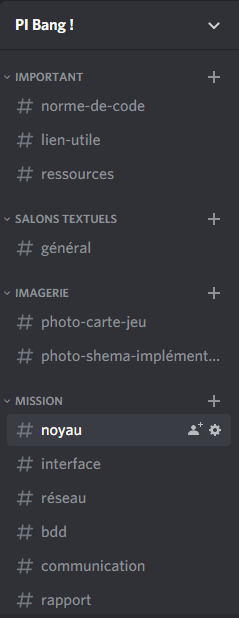
\includegraphics[width=0.48\textwidth]{Img/image4.png}
  \end{center}
  \caption{Différents salons}
\end{wrapfigure}


Nous avons utilisé dans notre groupe trois moyens de communication. 
D’une part, les réunions nous permettaient de discuter de l’avancée du projet de vive voix et de programmer la suite de l’organisation. Celles-ci étaient cruciales afin de communiquer l’avancée du projet et des attentes de chaque groupe par module. Les membres d’une équipe pouvaient ainsi expliquer leur travail à la cheffe de projet qui le notait et le comparait avec le planning prévu. \\ 




Ensuite, les différents outils de Git, les « issues » étaient utilisés afin de faire part aux autres membres de l’équipe des problèmes rencontrés dans le code et le « wiki »  rapportant les faits énoncés pendant les réunions. \\




Enfin ,Discord, notre outil principal, nous a permis de créer un serveur avec différents salons afin de pouvoir garder une trace écrite des conversations et de pouvoir communiquer rapidement et efficacement. De plus, Discord permet les conversations vocales et le partage d’écran, permettant la visualisation du travail d’un membre en direct. \\



Vous pouvez voir sur \textbf{la figure 1} les différentes catégories ainsi que les différents salons qui les composent. \\

\newpage

Nous avons ainsi pu mettre à jour les rôles d’un membre changeant d’équipe. Ce système était un moyen supplémentaire d’informations qui permettait à chacun de connaître, à tout instant, le statut des autres membres. Les rôles servaient également à contacter de façon exclusive les personnes travaillant avec nous.  En tapant « @IHM », par exemple, cela permet d’envoyer une notification de message uniquement aux membres du groupe “IHM” (\textbf{la figure 2 ci-dessus}) \\

Ce serveur discord nous permettait de discuter des différents avancements du projet et d’établir des listes des changement à effectuer. Avec la fonctionnalité d’épingler des messages, nous pouvons établir une liste et la garder accessible rapidement sans devoir la chercher. Nous avons notamment épinglé, de cette façon, les liens du google document ou encore du time sheet. \\


\begin{figure}
	\begin{center}
	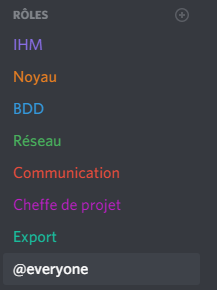
\includegraphics[width=0.48\textwidth]{Img/image5.png}
	\end{center}
	\caption{Exemple du @}	
\end{figure}


\newpage


\section{Le code}

\subsection{Le noyau du jeu}

\subsubsection{La première version du noyau}

Le noyau tel qu’il est décrit ici correspond à la version hors-ligne du noyau tel qu’il a été conçu au début du projet. Il a servi de base à l’équipe réseau qui l’a ensuite modifié à sa guise pour le faire fonctionner en ligne. Certaines informations ici sont donc obsolètes par rapport à la version finale du noyau. \\

\begin{enumerate}
	\item \textbf{La boucle principale} \\\\
	Lorsque le noyau du jeu est lancé, celui-ci crée le plateau : il instancie la classe board qui est le cœur du jeu. La classe board, lorsqu’elle est instanciée, crée et attribue les personnages et les rôles de manière aléatoire. Elle crée aussi le tableau de dés, utiles pour simplifier les interactions. Les instances de Player ont toutes accès au board (leur créateur) afin d’utiliser certaines méthodes.  \\
Une fois que tout cela est fait, les personnages et rôles attribués à chaque joueur sont révélés à ces derniers en créant un dictionnaire via la méthode reveal() de board et en l’affichant depuis le main. La boucle du jeu fonctionne comme suit : on demande à l’utilisateur quels dés il souhaite relancer (tous les dés sont automatiquement sélectionnés si c’est le premier lancer) et on lance la méthode playerAction de board qui s’occupe des effets immédiats tels que les flèches ou la dynamite. Les dés étant des dynamites sont bloqués et ne sont donc pas relancés même s’ils sont sélectionnés. Lors du passage au joueur suivant ils sont alors débloqués. Tant que le joueur qui joue a le droit de relancer les dés, ces opérations sont répétées. Si le joueur souhaite finir son tour, son nombre de lancers restants passe à 0 puis on effectue l’application des effets et on passe au joueur suivant. Si il meurt pendant son tour ou si il reçoit 3 dynamites, les effets ne sont pas appliqués (l’attribut de board silenced passe à 1 pour dire que les effets ne sont pas pris en compte). Cette dernière fonctionnalité a ensuite été changée dans la version en ligne du noyau car elle était dûe à une erreur dans la compréhension des règles. \\

\newpage

	\item \textbf{L’application des effets et cas de mort/fin du jeu} \\\\
	L’application des effets se fait par “effectsApplication” de “board”. Il regarde les dés et lance les méthodes appropriées pour que l’utilisateur fasse ce qu’il faut en fonction de ses dés. À chaque fois que des dégâts sont infligés à quelqu’un, un test de mort est effectué, méthode” testDeath” de plateau, sur ce joueur. S’il meurt, il est supprimé de la liste des joueurs et s’il était en train de jouer c’est alors la fin de son tour et ses effets s’arrêtent. Lorsqu’un joueur meurt, un test est lancé pour voir si la partie doit continuer ou non : “testEnd” de “board”. Si la partie doit se finir, l’attribut end de board est modifié en fonction du gagnant et la boucle du jeu s’arrête. \\



	\item \textbf{Les effets des personnages} \\\\
	Pour gérer les effets de personnages, la classe Player est héritée par chaque personnage jouable et certaines méthodes et/ou attributs sont modifiés, en fonction de leur caractéristique. Il n’est donc pas nécessaire de faire des tests à chaque fois pour savoir ce qui doit être fait en fonction des personnages en jeu. Chaque personnage est responsable de ses points de vie et de ses effets et le plateau ne fait que maintenir l’ordre et dire ce qui doit être fait.

\end{enumerate}

\subsubsection{Le noyau version finale}

	La première version du noyau était fonctionnel mais correspondait à une conception séquentielle et impérative alors que notre jeu en ligne est prévu pour être evenementiel.  Au moment de la mise en réseau on s’est rendu compte que le noyau qu’on avait conçu était parfait pour se jouer automatiquement mais qu’il était impossible d’interagir avec lui sans mettre en place de grosses dépendances. Cela l’aurait rendu très fragile. Ainsi il a été re-conceptualisé. \\
	 
	La version finale du noyau a été pensée pour correspondre à un ensemble d’objets qui en les associants permettent de symboliser une partie. Ainsi il correspond plus à une sorte de framework qui est utilisé par le serveur pour répondre aux requêtes des joueurs. Il est composé d’une représentation (classe) des dés, une des joueurs, une du plateau et enfin celle correspondant à un lobby (salon de jeu). La classe des dés et des joueurs n’a pas eu besoin de réel changement d'implémentation et la même idée que dans la première version a été retenue. Cependant celle représentant le plateau a dû être repensée entièrement. En effet plusieurs méthodes ont dû être décomposées en plus petites. Ainsi chaque action qui peut se faire sur un plateau de jeu a été implémenté sous forme de méthode.
	
\newpage

	 De cette façon on pouvait prendre le contrôle sur le jeu via un intermédiaire extérieure (Le serveur). Ainsi pour effectuer une application d'effet spécifique (choisie par un joueur) on peut l’effectuer directement grâce au serveur. \\
	
	La classe lobby elle a été ajoutée pour pouvoir distinguer les différentes parties qui peuvent être instanciées par le serveur et pour y associer un groupe de joueurs particuliers. Cette classe est donc plus comme une grosse interface entre le serveur et le noyau. Le serveur y trouve toutes les informations dont il a besoin pour les communiquer aux joueurs distants et le noyau y reçoit les différentes requêtes du serveur pour faire avancer le jeu.  \\
	


\subsection{L'IHM}


\subsubsection{Le Menu}

	Dans la conception du Menu, nous avons implémenté un menu simple d’utilisation
proposant un système de login au client. S’il est déjà inscrit dans la base de données, il devra renseigner son email ainsi que le mot de passe qu’il a enregistré lors de son inscription. \\

Dans le cas où le client n’est pas encore inscrit, il recevra une erreur, lui indiquant de s’inscrire via le formulaire présent. Si celui-ci n’est pas conforme, il devra alors rectifier les renseignements qu’il a précédemment fourni. Dans le cas où le client est inscrit et a donné les bonnes informations, il lui suffira d’appuyer sur un bouton en forme de flèche partant vers la droite. Il sera alors authentifié par la base de données, et sera mis en attente de partie. Il pourra alors voir le nombre de personnes qui patientent avec lui. \\

	Dans le cas d’une inscription, l’utilisateur devra fournir les informations suivantes :

\begin{itemize}
	\item pseudo : le nom qui le désignera durant ses futures parties.
	\item mot de passe : son code personnel de sécurité qui doit au moins comporter 6 caracters.
	\item confirmation du mot de passe : un code afin de vérifier que son mot de passe est bien celui escompté.
	\item mail : son adresse mail qui servira d’identifiant à la base de données. 	 \\
\end{itemize}


\newpage 

Si le client a fourni toutes ces informations sans erreurs, il sera alors redirigé vers le formulaire de connexion. Si en revanche le client a changé d’avis et ne souhaite pas s’inscrire, il pourra appuyer sur la flèche de gauche et retourner à la page d’accueil sans s'être inscrit. \\

En fonction des préférences du joueur, il pourra modifier le volume de la musique jouée en arrière plan grâce à un slider en bas à droite de l’affichage. Il pourra aussi modifier d’autres aspects du jeu en appuyant sur le bouton settings qui est indiqué en haut à droite sous forme de roue mécanique comme signe de configuration.

\subsubsection{Le plateau}

Dans la conception de l'IHM nous avons cherché la simplicité et avons donc opté pour une table où les cowboys s’assoient pour jouer. Cette table s'adapte au nombre de joueur, qui varie de 4 à 8. \\

Chaque joueur contient 3 labels, son nom, son nombre de point de vie et son nombre de flèche obtenu. Le rôle d’un joueur est représenté par une image cachée à tous sauf à lui-même. Un joueur incarne un personnage durant la partie de jeu. Celui-ci est indiqué par une image indiquant son effet spécial. \\

Les dés sont alignés au centre de l'IHM, associé avec un bouton “Rolldice” qui permet de lancer les dés, et un bouton “Activation effect” qui, comme le nom l'indique, active les effets des dés obtenus après leur lancé. Cette fonctionnalité est le point clé qui fera avancer la partie, c’est pour cela qu’il se trouve au centre. \\

À son tour un joueur doit sélectionner les dés qu'il souhaite relancer. Pour cela, il clique sur le bouton juste au dessus du dé choisi. une fois, tous les dés sélectionnés de cette manière, il peut les relancer en appuyant de nouveau sur le bouton “Rolldice”. \\

Il peut également annuler un choix en cliquant de nouveau sur le bouton au dessus du dé dont il désire annuler la sélection. Nous avons choisi cette démarche pour offrir un moment de réflexion au joueur afin de déterminer une bonne stratégie pour sa victoire. \\

Il est important, pour le joueur, de savoir le nombre de flèches restantes. À l’aide de cette information, il peut anticiper une attaque d’indien et établir une stratégie adéquate.  Il était donc nécessaire d’ajouter un affichage permettant de connaître à tout moment cette donnée.
 Les joueurs peuvent également adapter le son et d'autre options grâce au bouton settings identique au symbole de settings retrouvé au menu. \\
 
Quand un joueur A possède un personnage qui permet de choisir si on active son effet, et qu’il est attaqué par un joueur B, deux boutons “yes” et “no” et un label seront affichés. Ce label demandera au joueur s'il souhaite activer l’effet de son personnage ou pas. S’il n’a pas choisi, les boutons et le label disparaissent au bout de 5 secondes, et l’effet du personnage ne s’activera pas. 
Nous avons implémenté ce choix car nous avons voulu donner un effet de pression afin d'empêcher le joueur de faire attendre les autres indéfiniment, et accentuer la sensation de far-west “who is the fastest gunslinger?”. \\

Quand un joueur meurt, l’image de son personnage, de sa vie et de ses flèches, seront cachés par une image d’une tombe, et son rôle sera affiché à tout le monde. \\

Comme il est important que les joueurs puissent communiquer entre eux, nous avons ajouté une chatbox à côté du plateau, de sorte que chaque joueur puisse obtenir des informations importantes du serveur, mais également des messages d’autres joueurs afin de mieux planifier sa victoire.


\subsection{Réseau}

Le développement de l'architecture réseau a été pensée pour être la plus simple possible. L’objectif était de faire un jeu multijoueur avec un serveur centralisé. Or le moteur de jeu Godot a surtout un framework pour faire du peer-to-peer. C’est pour cela qu’il nous fallait une architecture épurée.  \\

Il s’agit d’une architecture basique serveur/client. Les clients communiquent avec un serveur hébergé sur google cloud et celui-ci transmet l’information au noyau pour effectuer la requête du client. \\

Ensuite il envoie des paquets à tous les clients en jeu. Ainsi, le plus important était de déterminer un protocole de communication. Pour cela nous avons décomposé les différentes phases de jeux (connexions/début de partie, distribution des rôles, La partie, Fin de partie). En partant de ce postulat, nous avons imaginé les messages qui pouvaient s’échanger.

\newpage


\subsubsection{Dans l'IHM}

Ayant établi la structure du réseau, il fallait adapter l'IHM en lui ajoutant des moyens de capter chaque message que le réseau devait lui envoyer. \\

Comme le réseau envoyait les informations telles que, la vie des joueurs, le nombre de flèches utilisées, les joueurs morts et leurs pseudonymes, il fallait que l’IHM reçoit et analyse ces informations afin d’adapter son affichage tout en prenant en compte le joueur actuel et ceux qui ne jouent pas.
L’IHM est également chargée d’envoyer des message afin de faire part au réseau, des choix effectués par le joueur. Cela peut être durant un lancé de dés, l’activation de l'effet d’un dé, ou encore lorsque le joueur a terminé son tour. \\

Ces messages permettent donc d’informer le réseau mais ils servent aussi à informer les autres clients de ces changements. Le réseau va les notifier de ces changements et envoyer les nouvelles données du jeu, telles que le nombre de flèches restantes sur le plateau, le nombre de points de vie de chaque joueur, les flèches qu’ils possèdent, ainsi que le nombre de lancer restant au joueur à chaque tour. \\

De même, pour le chat, le serveur transmet les messages écrits par le joueur. L’IHM sera alors chargée de les afficher chez chaque client, afin que les utilisateurs puissent discuter entre eux. \\
	
Le message est envoyé à tous les clients depuis le serveur, hormis celui qui l’a écrit. Son message sera affiché simplement en local, seuls les messages des autres joueurs lui seront transmis en réseau. \\

Quand un joueur A ne joue pas, il obtient des messages du réseau, tels que la modification des dés par un joueur B. Pour le joueur A, en attente de son tour, les boutons “Rolldice”, “Activate Effect” et “Endturn” ne seront pas affichés.


\subsubsection{Le serveur}

\begin{enumerate}
	\item \textbf{Choix d'implémentation} \\
	
	Le serveur est l’élément du jeu qui a été commencé le plus tardivement. Nos connaissances rudimentaires de l’utilisation de Godot et de l’architecture réseau, nous ont amenés à créer un plan de conception inadapté dans le cadre de notre projet. Nous avons donc mal défini les besoins auxquels nous devions répondre dans l’implémentation du réseau. Nous savions cependant que l’on souhaitait pouvoir l'implémenter en GDscript pour faciliter l’exportation du client par la suite. \\
	
Le jeu que nous souhaitions développer était un jeu de plateau au tour par tour. Les règles de celui-ci se devait d'être centralisées pour éviter les tricheries. Avec ces données en tête nous avons décidé de développer un serveur séquentiel et pouvant gérer plusieurs salon de jeu(parties).  \\

Le serveur a été fait de façon séquentielle pour faciliter son développement. L’implémentation d’un serveur fonctionnant de façon parallèle aurait été plus complexe à implémenter et aurait demandé des délais supplémentaires. Bang! étant un jeu de type “tour par tour”, cette implémentation, bien que optimale, n’est pas nécessaire au vu des  lourdes ressources qu’elle demanderait. \\

	
	\item \textbf{Évolution} \\
	
	Nous avions défini, sur papier, une architecture finale à atteindre. Étant donné que nous n’avions pas assez de compétences dans le domaine, il a été développé par tâtonnement.  Ainsi, nous somme arrivés à sa version finale en plusieurs étapes. \\
	
Dans un premier temps nous n’avions qu’un serveur qui pouvait accueillir 8 joueurs maximum et lancer une partie mais sans pouvoir répondre aux requêtes des clients. Après divers tests sur la réception des paquets et la mise en place du protocole de communication, nous avons implémenté la gestion des paquets envoyés par les clients. \\

Enfin nous avons réalisé l'implémentation des déconnexions imprévues. Cette étape fut complexe et nous avons dû surpasser beaucoup d’obstacles dans sa conception.   Il était en effet, très nuisible à l'expérience utilisateur, de se retrouver bloqué au cours d’une partie. Ainsi, nous avions une version du serveur plus stable et plus robuste.\\

Cependant cette version ne pouvait accueillir qu’une seule partie. Quand celle-ci était lancé, tout nouveau joueur se voyait déconnecté du jeu. Or notre objectif était d’avoir une version du serveur capable de supporter plusieurs parties en simultané. Dans cette optique, le serveur et le noyau (par l’ajout de la classe lobby) ont été retravaillés. \\

\newpage	
	
	\item \textbf{Décrire ses fonctionnalités finales} \\
	
	L’architecture du Serveur a été pensée pour être centrale au jeu et pour pouvoir gérer plusieurs parties en simultané. Ainsi le noyau, qui représente la partie, ne tourne que sur le serveur et reçoit des requêtes des joueurs pour effectuer des actions dans le jeu. \\

Cette architecture se base sur 4 caractéristiques:  \\

\end{enumerate}

\begin{enumerate}[label=(\roman*)]
	\item \textit{Gestion des connexions :} \\\\
	Quand un client se connecte le serveur doit enregistrer son adresse réseau puis l’affecter à un lobby (salon de jeu). Avant de lancer une partie, le serveur attend d’avoir rassembler suffisamment de joueurs dans un lobby. Une fois cette condition remplie, nous pouvons bloquer ce lobby puis initier une partie pour celui-ci. Ainsi un lobby est un objet ajouté au noyau pour que le serveur puisse gérer plus facilement plusieurs instances de jeu associer à un nombre de joueurs particuliers.\\

	
	\item \textit{Gestion des déconnexions imprévue :} \\\\
	Pour avoir une expérience utilisateur agréable et éviter qu’une partie soit bloquée à cause d’une déconnexion en cours de partie, nous avons décidé que toutes les déconnexions imprévues, entraînent la mort en jeu du déconnecté. Nous aurions pu choisir de laisser un délai à l’utilisateur pour se reconnecter. Malheureusement cela aurait été difficile car l’utilisation de trop nombreux signaux provoque une instabilité du serveur. Nous avons donc privilégié une implémentation moins riche mais stable.\\

	\item \textit{Gestion de la partie :} \\\\
	La gestion de la partie se fait en fonction des messages reçus. Le serveur, à la réception de chaque paquet, doit dans un premier temps identifier à quel lobby est associé le client qui lui a envoyé ce paquet. Ensuite, en fonction du message (voir messages), il effectue une action sur le jeu. Mise à part certains cas particuliers dûs aux effets spéciaux des personnages, il envoie en broadCast les nouvelles informations relatives à la partie.\\

\newpage

	\item \textit{Gestion de plusieurs parties en simultanées :} \\\\
	Afin de gérer plusieurs parties en même temps le serveur crée un tableau de lobby à l'initialisation du serveur. Quand quelqu’un se connecte au serveur il est placé dans le premier salon libre. Un dictionnaire est mis à jour avec l’adresse du client et l’indice du salon dans lequel il se trouve. Ce dictionnaire sert à identifier à quel salon correspond le message que le serveur vient de recevoir puisqu’il associe les différentes adresses des joueurs au salon dans lequel ils se trouvent. Si suffisamment de clients sont associés à un lobby, celui-ci peut commencer. \\


\end{enumerate}

\subsubsection{Les messages} 

Le protocole de communication mis en place pour communiquer entre les clients et le serveur découle des différentes phases de jeu qu’on a extrait des règles. Nous en avons décomposées 5. Ceci nous a poussé à créer 5 types de messages. De plus, puisque le nombre de messages et le contenu n’était pas très volumineux, nous avons décidé d’utiliser des chaînes de caractères comme moyen de transmission des informations. \\

	Toutes ces chaînes de caractères possèdent 2 types de séparateur. La virgule qui sépare des données (identifiant + valeur) ou des spécifications (définit le type de données qui va suivre) et les doubles points ( : ) qui séparent un identifiant de sa valeur. \\
	
	Pour rendre ces chaînes de caractères utilisables aisément, nous avons mis en place une fonction de parsing qui transforme ces chaînes en dictionnaires. Ainsi,il suffit de connaître la spécification et l’identifiant d’une donnée afin d’accéder à sa valeur.

En fonction de la phase dans laquelle se trouve le jeu, la partie, les messages qui doivent s’échanger entre le client et le serveur doivent être différents. Ainsi, pour pouvoir les différencier chaque chaîne envoyée doit commencer par un caractère spécial qui est considéré comme une spécification. \\


\begin{enumerate}
	\item \textbf{La connexion} \\
	En premier lieu il y a la connexion ou en terme du jeu décider à combien de joueur va se dérouler la partie. Dans cette phase les messages envoyés commencent toujours par un @. On peut y rencontrer seulement deux identifiants. \\
Alias et numberP qui respectivement prennent pour valeurs le pseudo du joueur connecté et le nombre de joueur connecté au lobby. Ainsi après la procédure de connexion le serveur peut envoyer le nombre de joueur et le client peut renseigner son pseudo. \\

Exemple :
@,numberP:3  --------> 3 joueurs dans ce lobby
@,alias:joueur3  ------> le joueur qui s’est connecté a pour pseudo joueur3 \\


	
	\item \textbf{La distribution des rôles} \\\\
	Les messages concernant cette partie commencent toujours pas ‘IN’. Ils sont composés de trois spécifications. Rôle, character et alias qui respectivement sont suivis de données représentant le rôle de chaque personne et celui qui possède le shérif, le personnage de chaque joueur et la communication de tous les alias. Une petite précision est de mise car pour garder le rôle des autres joueurs cachés on utilise la valeur Unknown. Cette partie n’est concernée que par le serveur. \\

Exemple avec 4 joueurs : \\
IN, \\
Role,0:unknown,1:Sherif,2:Hors-la-loi,3:Unknown, \\
Character,0:Suzzy,1:Pedro ramirez,2:willy the kid,3:Vulture Sam, \\
alias,0:J1,1:ALiAs,2:Hikaro,3:Gilfo \\

\newpage

	\item \textbf{La phase de jeu} \\\\
	Pendant la phase de jeu le serveur et les clients doivent s’échanger des messages complètement différents. Ainsi ils ont des spécifications complètement différentes. \\
		\begin{enumerate}[label=(\roman*)]
		\item \textit{Serveur :}\\
		
		Le serveur est celui qui sait qui est le client qui doit jouer. Ainsi nous avons décidé de commencer le paquet distribuant les informations concernant la partie par un caractère diffèrent en fonction de si il s’agit du joueur qui doit jouer ou non. \\
Si le client doit jouer alors il reçoit un paquet commençant par ‘~’ sinon par ‘!’. Ensuite ce paquet contient toutes les informations du jeu sous six spécifications: \\
	
	1 - Dice: contenant les faces actuelles des dés. (D,A,G,B,1,2) \\
	2 - HP:  Contenant les point de vie de chaque joueur \\
	3 - Arrow: Contenant les flèches reçues par chaque joueur \\
	4 - Throws: contient le nombre de lancés restants \\
	5 - Dead: Précise les joueurs morts (On révèle son rôle si c’est le cas) \\
	6 - Current: Précise le joueur qui joue en ce moment \\

	
Exemple pour 4 joueurs : \\

~, \\
Dice,0:D,1:A,2:G,3:B,4:G, \\
HP,0:3,1:2,2:4,3:2, \\
Arrow,0:3,1:0,2:0,3:1, \\
Throws,remain:2 \\
Dead,0:NO,1:Hors-la-loi,2:NO,3:NO, \\
Current,id:2 \\


\newpage
		
		\item \textit{Client:} \\
		
		Pour permettre au joueur de gagner, il fallait créer un message de modification des dés à chaque fois qu'ils étaient lancés. Le client envoie donc à chaque lancer les dés qu’il a sélectionné, sauf lors du premier lancement, où il est obligatoire de lancer tous les dés: \\

Exemple : \\
Rolling, \\
0:YES,1:YES,2:YES,3:YES,4:YES   --> le lancement de tous les dés. \\

Rolling, \\
0:YES,1:NO,2:YES,3:NO,4:YES → Lancement du premier, troisième et cinquième dés. \\

Une fois que le client A a terminé son tour, il envoie un message au serveur avec les dés activés. Dans le cas d’un dés qui devait cibler un joueur, il indiquera le numéro du dés, ainsi que l’identifiant du joueur. Si c’est un dés qui ne demande pas de sélection, alors il n’aura pas d’identifiant. \\

Exemple : Supposons que les valeurs des dés sont respectivements: B , 2 , 1 , D , A et que le joueur actuelle est le cinquième joueur. \\

 Dice,  \\
0:1,1:3,2:4,3:None,4:None → le client va guérir le joueur 1 avec la bière, il va attaquer le  
    troisième joueur avec le 2, il attaque le quatrième avec 1, et  
    les deux derniers dés ne sont pas des dés qui donnent la  
    possibilité de sélectionner un joueur. \\
    
\newpage

		

		\end{enumerate}
	
	\item  \textbf{La phase d’activation d'effets spéciaux} \\\\
	Toute la particularité de ce jeu réside dans les effets spéciaux des personnages. Ils contreviennent tous à certaines règles du jeu et certains d’entre eux ne sont pas automatiques. Ils nécessitent la décision du joueur. Ainsi il fallait un type de message qui demanderait au joueur d'effectuer une action alors que ce n’est pas son tour.  \\
	
La gestion des effets spéciaux se fait par l'intermédiaire de paquets commençant par le caractère \_ . \\

Exemple : \\
\_, \\
effect:Effet de bart  --> envoyé par le serveur pour notifier qu’il peut activer son effet \\

\_, \\
effect:Yes --> réponse du client concerné \\

	

	
	\item  \textbf{La gestion du chat} \\
	Pour permettre aux joueurs de communiquer entre eux nous avons aussi mis en place un chat. Ainsi tout paquet concernant le chat commence par le mot chat. \\


Exemple : \\

chat,text:Salut    --> client vers serveur (son pseudo jean) \\
chat,test:Salut,alias:jean --> serveur vers tous les clients de cette partie \\

	
 
	
	\item  \textbf{La gestion de fin de partie} \\
	Pour la fin de partie le serveur doit renseigner le rôle de tous les joueurs et quels joueurs ont gagné la partie. Ce type de paquet commence par le mot Victory. \\

Exemple : \\

Victory, \\
R,0:Sherif,1:Hors-la-loi,2:Hors-la-loi,3:Renégat, \\
V,0:Yes,1:NO,2:NO,3:NO \\

L’équipe du shérif a gagné. \\

	
\end{enumerate}


\subsection{La base de données} 


	La base de données a été faite sur Firebase qui est un moyen simple de créer des bases de données et de pouvoir la modifier via des requêtes http depuis un programme sur mobile ou pc. De plus, Firebase possède une documentation assez fournie ce qui nous a tout de suite attirés, elle  assure également toutes les fonctionnalités requises pour une base de données telles que l’inscription par mail ou par google play, par exemple, et de façon efficace, automatique (il suffit de connaître les requêtes associées) et sécurisée. Lors de la création d’un compte, Firebase crée un id pour le compte en question qui est utilisable ensuite pour définir la collection. Ainsi, Firebase est cross-plateforme : des utilisateurs sur mobile (google play) ou sur pc peuvent accéder à leur compte depuis ces deux plateformes. \\

\textit{Contenu de la table :} \\\\
	La table contient des collections, le modèle entités-associations que nous avons donné dans le premier rapport n’est donc pas applicable tel quel. En clair, la table contient une collection de joueurs “player” qui sont référencés par un id unique correspondant à celui fourni par Firebase lors de la création du compte. Chaque joueur possède un nombre de victoires “ wins“, de défaites “losses”, un pseudo “pseudo” et un booléen pour savoir s’il est en ligne ou non “online”. Il a en effet été décidé que nous ne ferions pas de liste d’amis, faute de temps, donc tout ce qui est en rapport avec la liste d’amis a été enlevé. Le booléen “en ligne” a été gardé car il est utile pour d’éventuelles versions futures incluant cette liste d’amis, car il permettra de savoir si un ami dans notre liste est actuellement connecté ou non. \\

\textit{Sign-in/sign-up :} \\\\ 
	Lorsqu’un utilisateur souhaite s’inscrire, il doit renseigner une adresse mail et un mot de passe. Firebase va ensuite automatiquement envoyer un mail de confirmation à cette adresse. Pour se connecter, il faut procéder de même. Les erreurs sont toutes prises en compte et l’utilisateur est prévenu s’il renseigne de mauvaises informations : mail inexistant, mot de passe ne correspondant pas à celui renseigné lors de la création du compte, mail n’ayant jamais été renseigné lors d’une création de compte etc…
Utilisation : l’utilisation de la base de données se fait en utilisant des requêtes http à des moments clés : lorsque la partie se termine, afin de modifier “wins” ou “losses”, lorsque l’utilisateur se connecte ou qu’il se déconnecte par exemple. \\

\newpage

\textit{Accès :} \\\\
Pour accéder à la base de données, il faut d’abord se connecter au compte google du groupe via l’adresse mail ci-dessous, car ce compte est le propriétaire de la bdd et peut donc y accéder et la modifier comme il l’entend. \\


Pour accéder à la base de données, il faut d’abord se connecter au compte google du groupe via l’adresse mail ci-dessous, car ce compte est le propriétaire de la bdd et peut donc y accéder et la modifier comme il l’entend. \\
\\
\textbf{Adresse mail :} pi.bang.groupe2@gmail.com \hfill  \\
\textbf{Mot de passe :} groupe2cd  \\
\textbf{Lien :} \url {https://console.firebase.google.com/u/0/project/pi-bang/database/firestore/data~2Fplayer~2FSnQARfjLrHHFEsAiEUb6~2Ffriends?hl=fr}  \\\\


\subsection{L’exportation}

Selon le cahier des charges, nous devions porter notre projet sur deux plateformes différentes. Godot met à notre disposition plusieurs options d'exportation afin de répondre à ce critère. Parmi ces options se trouvaient l’export Android et HTML5, parmi lesquels nous devions faire un choix, l’export iOS étant encore expérimental sur Godot. Samuel a été chargé de vérifier la viabilité de ces deux exports. \\ 

Notre choix se porta sur l’export HTML5 pour plusieurs raisons. Tout d’abord, l’export Android nous demandait plus de travail du côté de l’IHM, ce qui ne nous avantageait pas compte tenu du retard que nous avions accumulé au fil du projet. Une raison supplémentaire, et plus conséquentielle, est que la websocket du client Android ne parvenait pas à se connecter à la websocket du serveur depuis l’export Android, ce qui empêchait toute communication. Nous n’avons pas cherché à investiguer la cause de ce problème, puisque l’export HTML5 fonctionnait sans problèmes, nous orientant ainsi dans notre choix.  \\

\newpage

Afin de lancer cette version exportée du jeu en local, il nous faut servir le fichier html exporté via un serveur http. Ceci est nécessaire dû aux normes de sécurité des navigateurs, et peut être fait en exécutant la ligne suivante depuis un terminal (idéalement situé dans le répertoire de votre export) : 
\url{python -m http.server PORT --bind ADRESSE_IPv4} \\


 Puis en entrant l’url suivante dans votre navigateur :  \url{ADRESSE_IPv4:PORT} . Vous pouvez maintenant tester votre jeu, exporté en HTML5 dans votre navigateur \\

Néanmoins, cette solution d’export ne fonctionne que sur certains navigateurs, à savoir Google Chrome et Mozilla Firefox. L’export Godot repose en effet sur le support de WebAssembly par le navigateur hôte, que tous les navigateurs ne supportent pas à ce jour. Microsoft Edge le supporte, mais le jeu ne fonctionne néanmoins pas dessus. Safari fonctionne potentiellement puisqu’il supporte WebAssembly, mais ne possédant pas de machine Apple, ce dernier n’a pas pu être testé. \\

Au terme de ce projet, notre jeu fonctionne sous MacOS, Windows, Linux et dans les navigateurs internet susmentionnés.  \\
 
	
\section{Les perspectives}

\subsection{Améliorations du jeu}

Nous avons déjà en tête des améliorations possibles pour le jeu. Premièrement, nous pouvons finir d’ajouter tous les personnages présents dans le jeu originel, ce qui devrait nous demander environ 1 semaine, de plus nous pourrions créer et ajouter de nouveaux personnages qui ne sont pas présents dans le jeu de base, leur implémentation pourrait prendre également une semaine environ, en revanche leur création serait peut être plus longue puisqu’il faut réfléchir à des personnages qui n’aurais pas trop d’avantage vis à vis des autres. Nous pouvons également proposer différents styles graphiques ou musiques aux joueurs afin qu’ils puissent mieux s’approprier le jeu, cet ajout se ferait tout au long de la durée du jeu, avec des updates de temps en temps. \\

	Nous avions aussi prévu, pour des raisons de sécurité, d'intégrer la BDD dans le réseau au lieu de mettre les requêtes dans l’IHM, cela devrait prendre environ une semaine car il faudrait changer quelques messages qui sont envoyés au serveur, en effet il faudrait rajouter le mot de passe dans les messages envoyés, ou encore toute les infos lors d’une inscription. \\

L’architecture du serveur est encore perfectible. En effet cette version n’est pas faite pour un déploiement du jeu à très grande envergure.  \\
Il s’agit d’un serveur purement séquentiel. Il serait assez rapidement submergé par les requêtes. Une idée serait de créer un thread pour gerer chaque lobby ou chaque client. Cela nous permetrait ainsi de profiter de toute la puissance de la machine a disposition. Il serait tout aussi imaginable de changer pour une architecture de serveur distribué. Avec un serveur central pour la connexion. Celui-ci redirigeant les clients vers un autre serveur, hébergeant leurs parties. \\

Ensuite on se rend vite compte que ce jeu nécessite un nombre de joueurs minimum pour lancer une partie. Nous pouvons donc facilement imaginer qu’un joueur puisse se retrouver à attendre la connexion de suffisamment de joueur trop longuement. Il est possible de concevoir une IA permettant de remplacer les joueurs manquants.
Pour implémenter le serveur multithread plus serveur distribué il faudrait au moins 2
de travail à temps plein avec équipe de 3 ou 4 personnes. \\

Cependant cela reste dur à évaluer puisque ça nécessite de maîtriser de nouvelles notions de godot et de se documenter sur ce qu’est un thread safe ou pas.  \\


\subsection{L’extension}


Une extension de « Bang! Le jeu de dés » nommée « Old saloon » existe et pourrait donc être rajoutée au fur et à mesure dans le jeu une fois sorti. Dans cette extension il y a 5 modules différents qui peuvent être joués individuellement ou tous ensemble, cela implique donc que nous pourrions les ajouter module par module et maintenir un certain intérêt chez les joueurs. Nous pourrions également rendre ces ajouts payants individuellement ou avoir un pack qui regroupe tous ces ajouts. \\

	Voici à quoi correspond chacun des modules : \\
- La Grande Gueule et le Lâche : Rajoute deux dés en plus, à son tour un joueur devra choisir entre garder les 5 dés de bases ou prendre 4 dés de base plus un dé de cette extension, La Grande Gueule est le nom d’un de ces dés qui a pour but d’avoir des faces plus offensives tandis que le Lâche a des faces plus défensives. \\

\newpage

\begin{itemize}
	\item \textbf{La Flèche du Chef Indien :}\\
	
	Ajoute la Flèche du Chef Indien dans le tas de flèche, si un joueur choisit de prendre cette flèche, quand il doit prendre une flèche, lors d’une attaque d’Indien si il est celui avec le plus de flèche (pas d’égalité) il ne prendra aucun des dégâts causés par ces flèches, en contrepartie si il y a égalité ou que le joueur possède moins de flèches qu’un autre joueur alors cette flèche lui retire deux points de vie au lieu d’un. \\

	\item \textbf{Rôles spéciaux :} \\
	
	Rajoute des rôles spéciaux, il y a toujours les mêmes rôles sauf qu’ils ont également une capacité spéciale qu’ils peuvent activer une fois durant la partie, cela implique qu’ils révèlent leur rôle. \\

	\item \textbf{Une Clique de Nouveaux Personnages :} \\
	
	 Ajoute des nouveaux personnages dans le jeu, certains interagissent avec les autres modules et d’autres non. \\

	\item \textbf{Le Fantôme (utilisable à 5 joueurs ou plus) :}\\
	
	 Ajoute la carte du fantôme, le premier joueur à mourir devient un fantôme, il pourra à son tour lancer 2 dés de base et les lancer comme dans le jeu de base, cependant les effets des faces ne seront pas pour le joueur, il obligera un joueur à avoir les faces qu’il a obtenu après son lancé initial, cela peut donc être des effets positifs ou négatifs. \\

\end{itemize}


	Nous avons fait une estimation du temps qu’il nous faudrait afin d’ajouter les modules. Il faudrait compter 2 à 3 semaine pour le premier, 1 semaine pour le deuxième, 2 à 3 semaines pour le troisième, 1 semaine pour le quatrième et enfin 3 semaines pour le dernier. \\

\newpage

\section{Les apports individuels}



\subsection{Mathias Charpentier}


Dans ce projet, j’ai été chargé, à l’aide de plusieurs partenaires, de réaliser l’interface homme-machine du projet, de concevoir la base de données et sa mise en oeuvre et d’établir un plan de communication dans le but de donner de la visibilité au futur produit. \\

J’ai rédigé le cahier des charges du projet et réalisé l’UML du jeu et l’analyse S.W.O.T.
Ma participation à la réalisation de l’IHM n’a été que mineure. En effet, j’ai mis en relation à notre groupe de travail, un infographiste qui nous a permis d’améliorer certaines ressources graphiques élémentaires.
 Notre version numérique du jeu bang nécessitait d’utiliser des symboles propres au jeu et trouvable qu’en piètre qualité sur le net. Etant dans l’incapacité de pouvoir réaliser un traitement de l’image par manque de technique, nous nous somme allégés de cette charge de travail en ayant recours au soutien d’une personne capable de vectoriser des images afin d’en enlever le bruit. \\
 
Cette personne n’a aucunement participé à la réalisation d’animation ou d’outils de communication. Son travail s’est limité à l’amélioration d’éléments graphiques indispensables. \\

Aux prémices du développement, j’avais dans l’idée d’ajouter un mode solo à notre jeu. Lorsque la partie noyau fut implémentée et que l’ihm était en cours de développement, j’ai entrepris une intégration ihm-noyau dans le but de réaliser ce mode de jeu. \\

Cependant, après quelques jours de développement non concluant et le constat du manque de temps, nous avons pris la décision d’abandonner cette implémentation et de nous tourner vers une utilisation du jeu intégralement connectée. \\ 

J’ai alors travaillé sur la mise en place de la BDD hébergée sur Firebase. J’ai donc réalisé les fonctions d’enregistrements et de connexions, de stockage des données win/lose d’un joueur, de suppression de compte et de modification de pseudo. J’ai également réalisé des tests pour m’assurer que mes fonctions étaient bien résistantes. \\

Je me suis ensuite occupé de l’intégration de la BDD à l’aide de mes collègues. Cependant l’architecture du projet différait légèrement de mes attentes. J’ai donc isolé l’intégration de la BDD dans une nouvelle branche afin d’y effectuer des modifications. \\\\

 J’ai dû adapter mes fonctions pour les faire fonctionner avec l’implémentation en place. Cette étape a été retardée par l’apparition d’erreures largement imprévues.
Après avoir re-valider mon travail auprès de mes pairs, nous avons fusionner l’ihm en place avec la bdd. Ce “merge” n’a pas été sans conflits. Il nous a fallu tester longuement afin de nous assurer qu’aucun d’entre eux ne provoquerait d’erreurs fatales et difficilement solvables. \\
 
  Enfin, j’ai travaillé sur la mise en place de réseau sociaux, capables de promouvoir le produit et d’informer les différents utilisateurs des événements intérieurs et extérieurs au jeu (mises à jour, conventions, etc). J’ai réalisé le rapport de Communication avec l’aide de mes collègues qui ont chacun apporté une partie. J’ai pour ma part apporté la partie sur les réseau sociaux et co-écrit la partie sur les plateformes de distribution. J’ai également oeuvré dans la rédaction du rapport final ici présent ainsi que sa mise en forme. \\
  
\subsection{Elias Chetouane}

J’ai en premier lieu été affecté à l’équipe s’occupant du noyau. J’ai, à l’aide de mon équipe, écrit comment devait fonctionner le noyau dans son ensemble et d’un point de vue théorique. Lorsque nous sommes tombés d’accord sur son fonctionnement, nous nous sommes alors répartis les différentes classes à écrire et je me suis alors occupé de la classe du plateau de jeu (celle devant instancier les autres et les gérer) en extreme programming avec Nawfal. Une fois que toutes les classes ont été écrites, notre groupe a été dissous pour que chacun rejoigne d’autres groupes (sauf Nawfal et moi qui sommes restés sur le noyau) et je me suis alors chargé avec lui de la boucle principale (toujours en extreme programming), les effets de personnages et le fonctionnement global du noyau ainsi que de tester son fonctionnement. Le noyau a ensuite été rendu de manière à ce que tout puisse fonctionner en mode solo avec une mini-IHM faite rapidement (tout juste suffisante pour lancer une partie et tester les différentes fonctionnalités. \\

\newpage

Je me suis ensuite occupé de la base de données avec Mathias. Nous avons conçu la base de données sur Firebase et écrit le code permettant de l’exploiter. Pour cela nous avons utilisé le schéma entités-association apporté par Mike que nous avons dû adapter au fonctionnement un peu différent de Firebase. \\

Je me suis aussi occupé d’une partie de la communication : j’ai créé la page de présentation du jeu sur itch.io et développé cette partie du dossier de communication. Je me suis aussi renseigné sur d’autres plateformes sur lesquelles publier le jeu telle que Steam afin de comprendre leur fonctionnement et de savoir si cela valait le coup d’y ajouter le jeu. J’en ai alors déduit que la meilleure plateforme pour commencer restait itch.io et que cela ne valait pas le coup de le faire aussi sur d’autres (pour les raisons que j’ai développées dans le rapport concernant la communication). \\

Après tout cela, j’ai rejoint Nawfal pour finaliser l’IHM. Nous avons donc travaillé sur du débug ensemble pour la fin de ce projet, mais cela n’a pas aboutit à grand-chose. En effet, ceux-ci ne venaient pas de l’IHM. Nous nous sommes alors lancés en groupe sur la phase de test du jeu en rapportant les bugs que nous rencontrions. \\

Je me suis aussi occupé des différents rapports concernant le noyau en mode hors-ligne et la base de données, ces rapports sont disponibles dans ce fichier dans les parties dédiées. \\

Mention supplémentaire : vous vous demandez sans doute en lisant tout cela comment cela se fait que je prétends avoir contribué ainsi au projet sans rien avoir push sur git. Voici la raison : la plupart de mes travaux ont été réalisés en équipe d’au moins deux personnes (extreme programming), ou ne nécessitaient pas de push (la partie communication par exemple). Pour les travaux en extreme programming, je laissais la personne avec qui je travaillais faire les push. En effet, je ne suis vraiment pas familier avec la plateforme git et je travaille principalement sur mon ordinateur sous windows (pour tous les cours), et je n’ai donc pas vraiment pris le temps de comprendre comment git fonctionne sous windows, étant donné que son utilisation ne m’a jamais été indispensable. En revanche, je sais à peu près utiliser git sous linux, mais à partir du confinement je n’avais plus accès aux machines linux de la fac et j’ai alors préféré compter sur mes coéquipiers pour push ce que nous faisions. En effet, cela m’est égal de qui fait quel push tant que le projet avance. Je vous écris donc cela pour vous prévenir et en espérant ne pas être trop pénalisé pour mon manque d’utilisation de git (bien que j’utilise git pour récupérer les fichiers sur lesquels je dois travailler ou que je dois consulter bien entendu). \\

\subsection{Audrey Coeur-Joly}



En tant que cheffe de projet j’ai endossé le rôle tel qu’il est décrit dans la partie qui lui est consacrée.\\ 

	J’ai également réalisé l’explication la version texte des règles du jeu ainsi qu’en présentation vidéo et la réalisation des slides et textes pour les vidéos en me basant sur ce qui était écrit dans le rapport. J’ai voulu tourner les vidéos mais ayant mal à la gorge au moment de les tourner j’ai demandé à l’équipe de me remplacer, j’ai cependant quand même participé à la vidéo de démonstration et fait le montage des vidéos. J’ai écrit une grande partie des chapitres sur l’organisation et les futures améliorations possibles dans le rapport. J’ai également jugé bon de demander à des proches s’ils voulaient bien relire notre rapport afin de donner un point de vue extérieur. \\
	
	J’ai pris part à la rédaction de la communication en créant l’affiche et sa description en me basant sur l’image du menu. \\

	Afin de nous servir de modèle, j’ai aussi fournis le jeu “Bang! Le jeu de dés” lors des premières réunions afin de familiariser le groupe aux règles du jeu ainsi que de prendre les photos des différents éléments du jeu (dés et cartes) dans le but de les intégrer au projet. \\


\subsection{Ilias Deligiannis}

Pour ma part, dans ce projet, j’ai surtout participé à l'élaboration des fondations, de sorte qu'aucune partie de mon travail n’est visible directement par l’utilisateur. Dans un premier temps j’ai été affecté à l’équipe de développement du noyau. J’ai contribué à sa modélisation, conceptualisation et à une partie de son développement. Plus particulièrement j’ai implémenté le comportement des dés.  \\

Ensuite, j’ai changé d’équipe pour rejoindre celle du réseau. On a d’abord fait un travail de documentation pour trouver la technologie la plus appropriée pour son développement. Pour un export facile nous sommes partis sur l’utilisation des websockets. On a par la suite décidé de l'architecture de celui-ci, en équipe, puis il a été décidé que j’allais développer le serveur avec l’aide de Karim. J’ai ainsi commencé par imaginer tous les messages nécessaires au fonctionnement du serveur puis je les ai transmis à l’équipe du réseau travaillant sur l’IHM. \\

\newpage


Quand la phase de développement a commencé, nous avons remarqué que la conceptualisation du noyau n’était pas compatible avec l'architecture réseau que nous avions imaginé. De plus, le noyau était pensé pour un fonctionnement impératif alors que notre jeu se basait sur un concept évènementiel. Ainsi durant le développement du serveur avec Karim nous avons ré-implémenté le noyau. Dans un premier temps nous avons décomposé toutes les actions du jeu en différentes méthodes que le serveur peut appeler pour faire évoluer le jeu.  \\

Une fois ce problème résolu nous avons entamé le développement du serveur. J’ai mis en place la fonction du parseur pour rendre utilisable les paquets reçus, la procédure de connexion, la gestion des déconnexions imprévues, puis la gestion de l’application des effets des dés pendant que Karim s’occupait des autres fonctionnalités. Quand la première version stable du serveur fut délivrée, on pouvait faire tourner une seule partie sur le serveur, je me suis alors occupé seul d’améliorer le serveur pour que Karim puisse venir en aide à l’équipe d’IHM qui nécessitait plus de travail que prévu. Ainsi, je me suis occupé d'implémenter la possibilité pour les joueurs de choisir s'ils veulent activer les effets spéciaux de leurs personnages et de la gestion de plusieurs parties simultanées (multi lobby) en retravaillant le noyau et en lui ajoutant une classe lobby et en imaginant une nouvelle architecture serveur. \\

La dernière partie de mon travail a été de rendre le serveur robuste pour qu’il puisse tourner 24h/24 en faisant une grande quantité de tests et de debug.

\subsection{Karim Dellali}

Dans ce projet, j’ai pu prendre part au développement de plusieurs aspects du jeu Bang!. J’étais, dans un premier lieu, affecté à l’équipe d’implémentation du noyau, ayant contribué et participé à sa modélisation ainsi qu’une partie du développement de celui-ci, j’ai pour ma part implémenté la classe des joueurs. Une fois la conceptualisation terminée et  les bases de celui-ci établies, nous avons avec Ilias, laissé la suite/fin de l’implémentation du noyau aux autres, pour basculer sur la partie réseau.  \\

Après avoir fait des recherches concernant le réseau sur Godot, nous avons conclu que nous allions nous passer de l’API proposée, après nous être documentés sur le sujet, pour utiliser des fonctionnalités avec lesquelles nous sommes déjà familiers. \\

Nous étions donc après cela quatre membres sur la partie réseau, Ilias et moi s’occupant du développement serveur, ainsi que Samuel et Mike, qui étaient concentrés sur la partie IHM/Réseau.

\newpage

Une fois le fonctionnement pensé, ainsi que les communications entre le client et serveur imaginées, nous avons pu débuter leur implémentation. \\

Dans un premier temps, nous avons tout d’abord dû revoir la conception du noyau avec Ilias, car celui-ci n’était finalement pas adapté pour le jeu en réseau évènementiel. Nous avons adapté les fonctions de celui-ci de sorte que le serveur puisse les utiliser pour le bon déroulement de la partie. Comme fonctions à revoir, nous avions notamment l’attaque des indiens, ou le fait de passer au joueur suivant, en ajoutant un tableau pour y stocker les joueurs morts, etc… Comme évoqué plus tôt, il a fallu revoir l’ensemble des fonctions pour que cela puisse être implémenté de façon évènementiel. \\

Du côté serveur, j’ai donc contribué à la première version stable, avec par exemple la récupération des alias envoyés par chaque client pour l’attribution de ceux-ci dans la partie, ou dans l’envoi des dés obtenus par un joueur, tout en ajustant certaines fonctions du noyau pour le bon fonctionnement du jeu. \\

Le serveur fonctionnant correctement, avec l’envoi des messages au client se faisant correctement, et le noyau adapté au jeu en réseau, nous avons pu alors jouer une partie entière, ce qui était l’objectif voulu dès le départ, c’est à dire une première version stable. Une fois cet objectif atteint, étant donné la plus grosse charge de travail présente dans la partie de l’IHM/Client, j’ai alors rejoint ce côté du développement, pour une question d’efficacité et d’avancement. Ilias ayant été du même avis que moi, il s’est alors occupé de l’amélioration du serveur, des debugs, etc. \\

J’ai donc basculé dans la partie IHM/Réseau, avec Samuel et Mike, où j’ai pu contribuer aux debugs et à l’avancée de celle-ci. Nous avons pu continuer la suite du débogage via Discord, sur les salons vocaux pour le client et le serveur, ce qui fut d’une grande utilité pour le travail en commun. Nous avions pour habitude de faire des réunions vocales, pendant lesquelles nous testions les divers fonctionnalités du jeu, puis d’établir une liste des soucis à régler, comme rafraîchir à chaque lancer de dé les informations présentes sur l’IHM, attribuer le nombre de points de vie et de flèches correctement, améliorer le chat de la partie, etc... \\

\subsection{Steve De Rose}

Je n’ai en rien participé au projet. Ayant conclu après le semestre d’automne qu’il me serait impossible de fournir la charge de travail nécessaire à la réussite de deux licences. \\

\subsection{Samuel Dierstein}

Ma première tâche fut d’abord chargée d‘investiguer les options réseaux et de base de données  intrinsèques à Godot. Suite à ces recherches, nous avons décidé (bien que tardivement) de ne pas utiliser l’API de haut niveau proposée, mais de nous limiter à un fonctionnement que nous connaissions déjà, afin d’aller plus vite dans le développement. C’est à dire que nous avons choisi d’envoyer des messages sous forme de chaîne de caractères et de les analyser plutôt que de nous servir des RPC que Godot propose.  \\

Suite à cela, j’ai travaillé sur plusieurs parties de l’IHM, notamment la formation des paquets réseaux, et la redirection du flow du code via des signaux de global.gd vers Gameplay.gd et Chatbox.gd. Une bonne partie de mon travail s’est déroulée en coopération vocale avec Mike lorsque nous devions écrire les messages réseaux du côté de l’IHM vers le serveur, et Karim qui a basculé sur l’IHM une fois le serveur presque terminé, afin de résoudre le grand nombre de bugs restants sur l’IHM. Je n’ai pas beaucoup de commit pour ces raisons : beaucoup de travail en vocal (commit auxquels j’ai participé à l’écriture mais que d’autres ont push), beaucoup de travail de recherche et de test, hospitalisation d’un proche sur la fin du projet. \\

J’ai également été chargé de vérifier quels exports fonctionneraient  correctement en HTML5 et Android (plus de détails dans partie II.5 “L'exportation”). \\

Sur la fin du projet, j’ai contribué au refactoring du code, afin qu’il soit plus lisible, flexible, et moins prompt aux erreurs. 

\subsection{Mike Duran}

Mon investissement dans ce projet fut divisé en plusieurs parties, J'ai pris donc part dans le développement de la base de donnée, l'IHM, le réseau, ainsi que le noyau. \\

Mon travail dans le développement de la base de données consistait à lui offrir un design facile et efficace avant tout. J'ai ainsi écrit le modèle d'entité-association dont l'équipe de base de données s'est inspirée dans le développement de cette dernière. \\

Ayant accompli ma mission, je me suis ainsi focalisé sur la partie d'IHM de ce projet. Les travaux effectués dans cette partie consistaient à concevoir le wireframe du jeu avec Benjamin Dusterdiek, de le modifier après les discussions au sein de l'équipe et à concevoir les dés du jeu, en leur offrant un effet de lancement, incluant un moyen au joueur de finir son tour. \\

Une fois cette mission terminée, je me suis occupé du menu du jeu, en lui offrant un système de login au client, et de les stocker dans un fichier (en attendant la finition de la base de données), offrant un système de check-in et un empêchement de réécriture du login.
J'ai ajouté le moyen de modifier le son dans le jeu en fonction du besoin du joueur, intégrant également un moyen de communication entre eux, une chatbox. \\

Mon investissement dans la conception du plateau du jeu consistait à lui offrir le positionnement des personnages, l'adaptation de l'IHM en fonction du nombre de joueur, l’association des rôles des personnages,des caractères, des points de vies, des flèches et la possibilité de cibler un joueur en fonction de l'effet des dés, que le joueur A a sélectionné. J’ai également fait en sorte que la syntaxe à envoyer au serveur soit accessible. \\

	Il a aussi fallu que j'adapte la mort des joueurs, ce qui nécessitait une adaptation du ciblage du joueur B, en fonction des dégâts et de la guérison effectués par le joueur A.
	Dans le cas de la victoire de l'équipe des gentils ou des méchants, j’ai fait en sorte que la victoire soit affichée et que les noms des gagnants soient identifiés, tout en offrant un moyen de retourner au menu principal en fin de partie. \\
	
Je me suis occupé d'intégrer le moyen pour les joueurs, qui ont un personnage offrant l'option d’activer son effet, de l’utiliser, dans l’IHM. J’ai aussi ajouté un timer de 5 secondes, afin que le joueur ne réfléchisse pas infiniment au choix d’activer son effet ou pas : si le timer est écoulé et que le joueur n’a pas donné de réponse, alors l’effet ne sera pas activé. \\

	Ce qui me ramène à la partie réseau du projet : \\
	
Au sein de cette partie du projet, ma principale occupation était d'adapter l'IHM aux requêtes envoyées par le réseau, ce qui signifiait une grande modification de l'IHM afin que le client puisse envoyer des messages fonctionnels au réseau. \\

Je me suis aussi occupé de plusieurs problèmes venant avec la fusion de l'IHM et du réseau comme la modification des dés pour tous les clients qui sont connectés.
Mon travail dans le noyau se résume à analyser sa logique afin que l'équipe réseau puisse l'intégrer dans le réseau de manière fonctionnelle. \\

J'ai pu apporter un soutien pratique à mon équipe mais aussi constant et efficace afin de mener à bout ce projet ambitieux. \\


\subsection{Benjamin Dusterdiek}

J’ai principalement et quasi-exclusivement travaillé sur l’aspect IHM du jeu. \\

Tout d’abord, j’ai commencé, avec Mike Duran, par travailler sur les wireframes, afin d’avoir une idée générale de ce à quoi devait visuellement ressembler le jeu. Ces wireframes étant fini, j’ai pu dès lors me mettre à la création de l’IHM. Contrairement à ce que l’on pourrait penser, même si on est bien aidé par le logiciel, le code à concevoir est plutôt conséquent et demande travail et réflexion. Nous avons décidé de scinder notre jeu en plusieurs scènes : un menu d’accueil, d’où l’on pourrait se connecter et lancer le jeu, un menu d’options, un menu “lobby”, c’est-à-dire une sorte de file d’attente où l’on pourrait voir la liste des parties, et enfin, la scène du jeu en lui-même, la plus importante. \\

Nous avons eu l’idée d’un menu simple, avec un champ pour le pseudo, un pour le mot de passe, et quatre boutons, un pour lancer le jeu, un autre pour créer son compte, un troisième pour ouvrir le menu d’options, et un bouton pour quitter le jeu. J’ai créé un menu relativement basique avec les fonctions principales de connection qui aura été graphiquement amélioré par Nawfal (les fonctions auront été modifiés, les premiers tests ayant été fait en local, pour coller à l’intégration de la BDD)
Le menu d’options est relativement basique - nous n’avions pas besoin de grandes quantités d’options pour notre jeu - et permet de choisir la langue du menu ainsi que le mode d’affichage. \\
Concernant le lobby, j’ai eu deux idées en tête, et j’ai finalement choisi la méthode que l’on a appliqué, à savoir une page où l’on pourrait choisir d’héberger une partie ou d’en rejoindre une, via des “cases” où l’on connaîtrait le nombre de joueurs dans la partie ainsi que son hôte. Au final, le lobby sera complètement remanié pour mieux coller à la vue d’ensemble de notre jeu. \\

Enfin, pour la scène de jeu : \\

Nous sommes partis sur l’idée d’une table autour de laquelle se situerait les joueurs, tout comme pour le jeu de plateau, mais également pour reproduire la vie typique des saloons que l’on voit dans les westerns où les gens se regroupent pour des parties de poker. J’ai mis en place avec la disposition des joueurs autour de la table ainsi que les informations liées à chaque joueur, tels que le nombre de points de vie ou son pseudo, ainsi que les prototypes des fonctions d’attaque et “de flèche”. Je me suis aussi occupé de l’agrandissement des cartes de joueur lorsque l’on clique dessus afin que l’on puisse confortablement lire les informations de la carte. L’intégration des dés dans la scène de jeu fut effectuée par Mike. \\

J’ai également effectué deux ou trois tâches annexes, telles que faire un début de système de création de compte (via un dictionnaire comprenant le pseudo et le mot de passe de la personne) qui aura servi de squelette au système de compte qui aura été mis en place, et créer des fonctions permettant de tester si les informations rentrées sont conformes à la convention “habituelle” : il fallait interdire certains caractères spéciaux pour le nom du joueur, son mot de passe, et son e-mail (tels que le slash ou les lettres diacritiques), ainsi que vérifier que l’adresse e-mail est conforme à la forme nom@adresse.nom-de-domaine.\\

Enfin, dans les dernières semaines, j’ai participé à l’intégration de la BDD avec Mathias Charpentier et Elias Chetouane, puis ai aidé Mathias sur les corrections des différents rapports. \\

\subsection{Nawfal Eddaoudi}

Tout d'abord, j'ai été affecté à l'équipe de développement du noyau qui comprend Elias, Ilias et Karim. Avec ces derniers, on a modélisé et conceptualisé le noyau tout en se partageant les tâches. En extreme programming, nous nous sommes occupés avec Elias de la classe du plateau. \\

Dès lors, après que toutes les classes ont été écrites par les membres de l'équipe noyau; celles-ci ont été changées, du fait que moi et Elias sommes restés dans le noyau pour se charger du fonctionnement global du noyau, ainsi que ses tests unitaires. Dans ce travail en extreme programming, je me suis chargé principalement des commit en précisant le binôme dans ce dernier. \\

Ensuite, j'ai été intégré à l'équipe IHM, où j'étais chargé d'améliorer le plus possible l'ensemble de l'IHM. Ayant une perspective différente au niveau design, j'ai pris la décision de refaire les wireframes, ainsi que d'améliorer l'ensemble des fonctionnalités non seulement d'un point de vue visuel, mais aussi fonctionnel (au niveau du menu des options, ou encore une animation dès l'ouverture du menu d'inscription etc) ;  en partant certes, du travail de Benjamin et en se servant l'image de l'infographiste sur l'arrière-plan du menu. \\

Une fois l'accomplissement de ces tâches, je me suis concentré essentiellement sur la scène du jeu, pour aider le maximum possible à son bon fonctionnement en améliorant du mieux que je pouvais le visuel du plateau pour une meilleure jouabilité (boutons/chat/recherches d'icônes et de musiques, etc). Puis, des ajouts importants des scènes (les options gameplay, l'écran de victoire etc). Mais principalement, un temps important a été consacré à identifier les bugs pour en trouver des solutions.\\


\newpage

\section{Remerciements}

Nous aimerions remercier notre professeur Stéphane Cateloin pour nous avoir accompagné tout au long de ce projet.  \\
Nous remercions également Thomas Hertrich qui nous a fourni quelques images de qualité pour notre projet et qui a retouché les images des dés.  \\
Et pour finir, nous remercions Benjamin Dujardin, Rémy Fayard, Mélanie Messager, Arthur Rauch et Louis Thomann pour avoir eu le courage de bien relire notre rapport. \\

\section{Conclusion}

Durant ce long projet, nous avons eu l’occasion de nous familiariser avec un nouvel outil de développement, Godot Engine, et de découvrir la programmation d’un jeu de plateau de sa conception à sa programmation. Nous n’avions jusque-là pas encore travaillé avec un groupe aussi conséquent. Cela nous a permis d’apprendre à améliorer notre communication et à écrire un code plus propre et compréhensible, facilitant la lecture de nos collègues. Nous avons réalisé également à nos dépends, qu’il est crucial  à ne pas se lancer dans l’implémentation avant de savoir comment fonctionnera chaque différent module du projet, car c’est ce qui nous a le plus retardé. \\

	Après les différentes épreuves que nous avons traversé nous avons gardé le moral afin d’obtenir un jeu fonctionnel et jouable auquel nous sommes contents d’avoir participé.



\end{document}
